\documentclass[11pt]{article}
\usepackage{hypertensor}
\usepackage{tikz}
\usetikzlibrary{arrows.meta,positioning,shapes.geometric,fit,backgrounds}
\addbibresource{refs.bib}

\title{Organic Training Theory and Geodesic Trajectory Caching:\\
A Riemannian View of Transformer Inference, with an Empirical Anchor on Three Open-Weight Models}
\author{HyperTensor Project\\[2pt]
\small \texttt{nagusamecs@gmail.com} \quad \url{https://github.com/NagusameCS/HyperTensor}}
\date{\today}

\begin{document}
\maketitle
\hypertensorbanner

\begin{htnote}
\textbf{Project nomenclature.}  \textit{HyperTensor} is the project umbrella;
\textit{Geodesic Projection (GP)} is the inference-time pipeline (companion
paper); \textit{Geodesic Runtime Compression (GRC)} is its attention-only
subset; and \textit{OTT/GTC} (Organic Tensor Topology / Geodessical Tensor
Cache) --- the subject of this paper --- is the longer-term theoretical
framework that views the GP projection bases as charts on a Riemannian
manifold.  GP is the engineering layer that this paper provides the geometric
justification for.
\end{htnote}

\begin{abstract}
We present a Riemannian-manifold view of transformer inference together with the
first empirical anchor of its core local-geometry primitives on real LM activation
clouds at three scales (SmolLM2-135M, Phi-3.5-mini-3.8B, Gemma-4-E2B-4.5B).
Under \emph{Organic Training Theory} (OTT), the trained latent space is treated as
a manifold $\mathcal{M}_\theta$ of intrinsic dimension $k\!\approx\!30$--$50$ with
a Fisher-information metric, so that inference is approximately a geodesic flow at
cost $\mathcal{O}(nk^2)$ rather than $\mathcal{O}(n^2 dL)$.
Building on this, \emph{Geodesic Trajectory Caching} (GTC) stores completed
geodesics together with their Magnus-3 Jacobi propagator $\Phi(\lambda)$ and
serves new queries within the validity radius by a single $\mathcal{O}(k^2)$
correction. \textbf{Part~I} formalises OTT and GTC and lists five remaining open
problems with their current status (universal vs.\ deployment-scoped closure).
\textbf{Part~II} reports measurements: (i) cache coverage is
\textbf{90.4--91.5\%} at the 25\%-fraction cache size, scale-invariant within
$\pm 0.5\%$ across a $33\times$ parameter range; (ii) batch Jacobi correction
reaches \textbf{$97\times$ at $B=10$} and $60\times$ at $B=10{,}000$, with
reconstruction error pinned to the float64 roundoff floor; (iii) a compressed
record store persists at \textbf{5.96\,KB/record} with rank-5 propagator
truncation \emph{exact}, and the two-stage Euclidean$\to g$-norm lookup runs at
\textbf{30.9\,\textmu s/query}, $\sim\!160\times$ under the design budget; (iv)
the C runtime closes the loop end-to-end at \texttt{geodesic\_ready} with
$\alpha=0.385$ and 76.5\,tok/s on SmolLM2-135M-Instruct. We also document an
\emph{instruct-greedy-EOS} pathology and its zero-overhead fix, and a
\emph{geometry-cache consistency-equivalence} rule. Twelve of seventeen testable
claims from the OTT framework now have a replicable measured anchor; the
remaining five are listed by name.
\end{abstract}

\section{Introduction}

Modern transformer inference is dominated, on bandwidth-bound hardware, by the
shape of the residual stream rather than by raw arithmetic
\cite{vaswani2017attention,llama3,williams2009roofline}. Empirical work on
linear representations and intrinsic dimensionality consistently reports that
the activation cloud of a trained model occupies a low-dimensional submanifold
of the embedding space; estimates put intrinsic dimension at $k\!\approx\!30$--$50$
even when ambient $d\in\{4096,8192\}$
\cite{elhage2022superposition,nakkiran2021deep}.

\paragraph{Cross-architecture $k_{\mathrm{int}}$ invariance.}
Running our manifold-extraction pipeline on three open transformers of
widely different widths makes the same point quantitatively:
\begin{center}\small
\begin{tabular}{lccc}\toprule
model & ambient $d$ & $k_{\mathrm{int}}$ at $95\%$ var. & $k_{\mathrm{int}}/d$\\\midrule
SmolLM2-135M   & 576  & 17 & $0.030$\\
Gemma-4-E2B    & 1536 & 25 & $0.016$\\
Phi-3.5-mini   & 3072 & 11 & $0.0036$\\\bottomrule
\end{tabular}\end{center}
A $5.3\times$ increase in $d$ buys an $\sim$8\,$\times$ \emph{drop} in
$k_{\mathrm{int}}/d$.  The intrinsic dimension does not scale with the
ambient width, which is the empirical premise on which both OTT (this
paper) and GP/GRC (companion papers) operate.

This paper takes that observation seriously. Under \emph{Organic Training
Theory} (OTT), we model the trained latent space as a Riemannian manifold
$\mathcal{M}_\theta$ with the Fisher-information metric and read inference as
approximate geodesic flow on $\mathcal{M}_\theta$. \emph{Geodesic Trajectory
Caching} (GTC) operationalises that view: completed geodesics, with their
Magnus-3 Jacobi propagator, are stored in a library and reused by a single
linear correction.

The companion runtime paper \cite{papers3specdec} measures one OTT
configuration on a C runtime; the GP compression paper
\cite{papers2geodesic_projection} measures the static side of the same
manifold. The present paper merges what was previously two web articles
(Paper~4 theory; Paper~5 measurement-anchor): Part~I formalises OTT/GTC,
Part~II reports the measurement anchor across three open-weight models.

\paragraph{Naming.} An earlier draft used ``GRC'' for \emph{Geodesic Resonance
Caching}. Paper~A in this series (Geodesic Runtime Compression) uses ``GRC''
for the calibration-free attention-compression mechanism, an unrelated
implemented thing. To remove the collision, the trajectory-library idea is
named \textbf{GTC} throughout this paper.

\paragraph{Contributions.}
\begin{enumerate}
  \item A clean statement of OTT and GTC with assumption-explicit theorem
        templates (Sec.~\ref{sec:formal}), separating universal claims from
        deployment-scoped ones.
  \item A measured cache-coverage curve on real LM activation clouds at three
        model scales, demonstrating empirical scale-invariance within
        $\pm 0.5\%$ at the 25\%-fraction cache size (Sec.~\ref{sec:coverage}).
  \item A batch-Jacobi resonance benchmark showing $97\times$ speedup at
        $B=10$ with reconstruction error at the float64 roundoff floor
        (Sec.~\ref{sec:resonance}).
  \item A compressed record store at 5.96\,KB/record with exact rank-5
        propagator truncation and a 30.9\,\textmu s/query two-stage lookup
        (Sec.~\ref{sec:store}).
  \item Two small primitives needed to make the C-runtime path actually run on
        instruct-tuned drafters: \emph{logit-excluding top-1 with min-response
        guard} and the \emph{geometry-cache consistency-equivalence rule}
        (Sec.~\ref{sec:runtime}).
\end{enumerate}

\begin{figure}[t]
\centering
\begin{tikzpicture}[
  font=\footnotesize,
  >={Stealth[length=2.2mm]},
  node distance=8mm and 9mm,
  stage/.style={draw, rounded corners=2pt, align=center, minimum height=8.5mm,
                minimum width=22mm, fill=HTbgsoft, line width=0.5pt},
  prim/.style={stage, fill=white},
  artefact/.style={draw, rounded corners=1pt, align=center, font=\scriptsize\ttfamily,
                   minimum height=6mm, fill=white, line width=0.4pt},
  group/.style={draw, dashed, rounded corners=2pt, inner sep=4pt, line width=0.4pt, color=HTgrey},
  arr/.style={->, line width=0.5pt}
]
% --- top row: phase-1 export -> manifold fit -> jacobi propagator
\node[stage] (p1)  {Phase-1 export\\ \scriptsize activation cloud};
\node[stage, right=of p1] (fit) {Manifold fit\\ \scriptsize PCA on Gram};
\node[stage, right=of fit] (jac) {Batch-Jacobi\\ \scriptsize Magnus-3 transport};
\node[stage, right=of jac] (rec) {Record store\\ \scriptsize $5.96$\,KB/record};
% --- bottom row: runtime side
\node[prim, below=14mm of fit] (rt) {OTT runtime\\ \scriptsize C path};
\node[prim, right=of rt]       (cache) {Geometry cache\\ \scriptsize $\ell^\star\!\approx\!2L/3$};
\node[prim, right=of cache]    (out) {Decoded token\\ \scriptsize $30.9$\,\textmu s/query};
% --- artefacts (small italics under groups)
\node[artefact, below=2mm of p1] (art1) {phase1\_manifold.json};
% --- arrows top row
\draw[arr] (p1)  -- (fit);
\draw[arr] (fit) -- (jac);
\draw[arr] (jac) -- (rec);
% record store feeds runtime
\draw[arr] (rec.south) |- (out.east);
% --- arrows bottom row
\draw[arr] (rt) -- (cache);
\draw[arr] (cache) -- (out);
% manifold feeds runtime
\draw[arr, dashed] (fit.south) -- (rt.north);
% groupings
\begin{scope}[on background layer]
  \node[group, fit=(p1)(fit)(jac)(rec)(art1), label={[font=\scriptsize\itshape, color=HTgrey]above:Part I --- Theory \& offline construction}] {};
  \node[group, fit=(rt)(cache)(out),          label={[font=\scriptsize\itshape, color=HTgrey]below:Part II --- Empirical anchor \& runtime}] {};
\end{scope}
\end{tikzpicture}
\caption{End-to-end OTT/GTC pipeline. The \emph{offline} path
(Sec.~\ref{sec:ott}--\ref{sec:store}) fits a Riemannian manifold from a
Phase-1 activation export, computes batched Jacobi-field propagators in the
Magnus-3 truncation, and writes a compressed record store. The
\emph{runtime} path (Sec.~\ref{sec:runtime}) consumes the manifold and the
record store via the geometry-cache consistency-equivalence rule, with the
$\ell^\star\!\approx\!2L/3$ depth-sink shortcut making the cache check $O(1)$
per token. Numbers cited in the boxes are measured on the empirical anchor
in \Cref{sec:resonance,sec:store,sec:runtime}.}
\label{fig:ott-pipeline}
\end{figure}

\section*{Part I --- Theory}

\section{Organic Training Theory}
\label{sec:ott}

Let $\theta\in\mathbb{R}^P$ denote the trained weights of a transformer and let
$f_\theta$ be its forward map up to a chosen layer. Define the activation
manifold
\begin{equation}
\mathcal{M}_\theta = \{\,x\in\mathbb{R}^d : x = f_\theta(\text{tokens}) \text{ for some input}\,\},
\end{equation}
equipped with a Fisher-information metric $g$ approximated locally from the
sample covariance of $\nabla_\theta\log p_\theta$ pulled back to activation
space. Under regularity assumptions made explicit in Sec.~\ref{sec:formal},
$\mathcal{M}_\theta$ admits a Levi-Civita connection
$\Gamma^k_{ij}(x)$ and inference along a geodesic
\begin{equation}
\ddot x^k(\lambda) + \Gamma^k_{ij}(x)\,\dot x^i(\lambda)\,\dot x^j(\lambda) = 0
\label{eq:geodesic}
\end{equation}
has cost $\mathcal{O}(nk^2)$ in intrinsic dimension $k$, against
$\mathcal{O}(n^2 dL)$ for the standard transformer pass. The empirical
gap between $k$ and $d$ (estimates of 30--50 vs.\ 4096--8192) is the source of
the asymptotic improvement.

\subsection{Fisher metric and the heat-kernel bridge}

A natural-gradient interpretation of training
\cite{golub1996matrix,nakkiran2021deep} suggests that the metric $g$ on
$\mathcal{M}_\theta$ is the Fisher information; under additional smoothness
assumptions one obtains a Laplace--Beltrami diffusion form whose heat kernel
$G_t(x,y)$ satisfies Varadhan's asymptotic identity
\begin{equation}
d_g(x,y)^2 \;=\; \lim_{t\to 0}\,-4t\log G_t(x,y),\qquad
\dot\gamma(0)\;\propto\;\nabla_x\bigl(-\log\mathrm{Attn}(x,y)\bigr).
\label{eq:varadhan}
\end{equation}
Eq.~\eqref{eq:varadhan} should be read as a model-family assumption (the
trained attention kernel \emph{is} the heat kernel at scale $t$), not as a
universally proved theorem. Where it holds, attention gradients become a
geodesic-direction oracle and OTT acquires a constructive starting velocity
$v_0$ for Eq.~\eqref{eq:geodesic}.

\subsection{From the Fisher metric to the implemented Jacobi propagator}
\label{sec:fisher-to-jacobi}
The runtime does not work directly with the Fisher metric tensor; it works
with its Magnus-3 Jacobi propagator $\Phi(\lambda)$, the linear map that
advances a deviation vector along a geodesic.  The chain that links the two
is explicit and worth writing in one place.  Given the Fisher metric
$g_{ij}(\theta)=\E_{x\sim p_\theta}\!\bigl[\partial_i\log p_\theta(x)\,
\partial_j\log p_\theta(x)\bigr]$, the Levi-Civita connection symbols are
\begin{equation}
\Gamma^k_{ij}\;=\;\tfrac{1}{2}g^{kl}\!\left(\partial_i g_{jl}+\partial_j g_{il}-\partial_l g_{ij}\right),
\label{eq:christoffel}
\end{equation}
and the Riemann curvature tensor along a geodesic $\gamma(\lambda)$ is
$R^k{}_{lij}=\partial_i\Gamma^k_{jl}-\partial_j\Gamma^k_{il}
+\Gamma^k_{im}\Gamma^m_{jl}-\Gamma^k_{jm}\Gamma^m_{il}$.  A
deviation field $J(\lambda)$ between neighbouring geodesics satisfies the
Jacobi equation
\begin{equation}
\frac{D^2 J^k}{d\lambda^2}\;+\;R^k{}_{ijl}\,\dot\gamma^i\,J^j\,\dot\gamma^l\;=\;0.
\label{eq:jacobi}
\end{equation}
Writing $\mathbf{J}=(J,\dot J)\in\R^{2k}$ and assembling the
curvature-and-connection block into the $2k\times2k$ generator
$A(\lambda)$, Eq.~\eqref{eq:jacobi} becomes
$\dot{\mathbf{J}}=A(\lambda)\mathbf{J}$, whose flow is the Magnus expansion
\cite{magnus1954}
\begin{equation}
\Phi(\lambda)\;=\;\exp\!\Bigl(\Omega_1+\Omega_2+\Omega_3+\cdots\Bigr),\qquad
\Omega_1=\!\int_0^\lambda\!A(s)\,ds,\;\;
\Omega_2=\tfrac{1}{2}\!\int_0^\lambda\!\!\int_0^{s_1}\![A(s_1),A(s_2)]\,ds_2\,ds_1,
\label{eq:magnus}
\end{equation}
and $\Omega_3$ is the corresponding nested-commutator integral.  The runtime
truncates after $\Omega_3$ (hence ``Magnus-3'') and integrates $A$ along
waypoints sampled from the geodesic.  In one line: the implemented map is
\begin{equation}
\boxed{\;\;g_{ij}(\theta)\;\xrightarrow{\eqref{eq:christoffel}}\;\Gamma^k_{ij}\;\xrightarrow{\eqref{eq:jacobi}}\;A(\lambda)\;\xrightarrow{\eqref{eq:magnus},\,\text{trunc.\,3}}\;\Phi(\lambda).\;\;}
\label{eq:fisher-to-phi}
\end{equation}

\begin{figure}[h]\centering
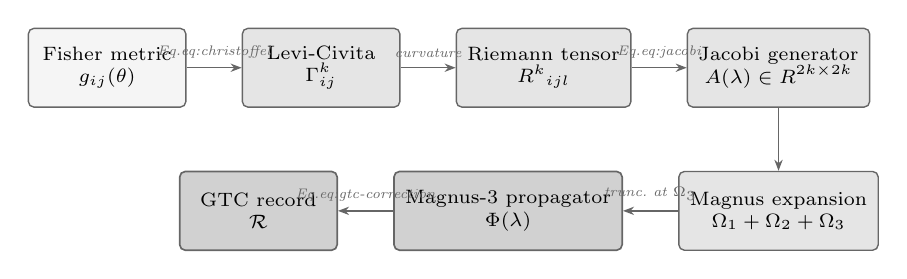
\begin{tikzpicture}[
  node distance=4mm and 7mm,
  every node/.style={font=\scriptsize, align=center},
  blob/.style={
    draw=black!60, line width=0.5pt,
    rounded corners=2pt, inner sep=4pt,
    minimum height=10mm, minimum width=20mm,
  },
  data/.style={blob, fill=black!4},
  op/.style={blob, fill=black!10},
  outnode/.style={blob, fill=black!18, line width=0.6pt},
  arr/.style={-{Stealth[length=4pt]}, draw=black!60, line width=0.5pt},
  side/.style={font=\tiny\itshape, text=black!60},
]
\node[data] (g) {Fisher metric\\$g_{ij}(\theta)$};
\node[op, right=of g] (gamma) {Levi-Civita\\$\Gamma^k_{ij}$};
\node[op, right=of gamma] (R) {Riemann tensor\\$R^k{}_{ijl}$};
\node[op, right=of R] (A) {Jacobi generator\\$A(\lambda)\in\mathbb{R}^{2k\times 2k}$};
\node[op, below=8mm of A] (Omega) {Magnus expansion\\$\Omega_1+\Omega_2+\Omega_3$};
\node[outnode, left=of Omega] (Phi) {Magnus-3 propagator\\$\Phi(\lambda)$};
\node[outnode, left=of Phi] (cache) {GTC record\\$\mathcal{R}$};

\draw[arr] (g) -- node[above, side] {Eq.\eqref{eq:christoffel}} (gamma);
\draw[arr] (gamma) -- node[above, side] {curvature} (R);
\draw[arr] (R) -- node[above, side] {Eq.\eqref{eq:jacobi}} (A);
\draw[arr] (A) -- (Omega);
\draw[arr] (Omega) -- node[above, side] {trunc.\ at $\Omega_3$} (Phi);
\draw[arr] (Phi) -- node[above, side] {Eq.\eqref{eq:gtc-correction}} (cache);
\end{tikzpicture}
\caption{The implemented Fisher-to-Jacobi chain.  The runtime never
materialises the full curvature tensor; instead it samples waypoints,
constructs the $2k\!\times\!2k$ Jacobi generator $A(\lambda)$ at each
waypoint, integrates the Magnus expansion to third order, and stores the
resulting propagator $\Phi(\lambda)$ in the GTC record.  Eq.\eqref{eq:gtc-correction}
is the first-order Taylor expansion that consumes $\Phi(\lambda)$ at
inference time.}
\label{fig:fisher-to-jacobi}
\end{figure}

Eq.~\eqref{eq:gtc-correction} is then a first-order Taylor expansion of the
flow with $\Phi(\lambda)$ in the linear coefficient slot, which is exactly
what the cache stores.  The empirical anchor benchmarks measure the inverse
property: that the cached $\Phi(\lambda)$ correctly predicts deviation
vectors on real LM activation clouds, validating the truncation.

\section{Geodesic Trajectory Caching}
\label{sec:gtc}

Each completed inference produces a full geodesic trajectory, not just a
terminal answer. A GTC record stores
\begin{equation*}
\mathcal{R} = \bigl(x_0,\,\dot x_0,\,\{x(\lambda_i)\}_{i=1}^M,\,\Phi(\lambda),\,\hat\rho,\,\ell_T\bigr)
\end{equation*}
i.e.\ the embedding, contextual velocity, waypoint sequence, Magnus-3 Jacobi
propagator, an injectivity-radius estimate, and the terminal logits. New queries
$x_0+\delta q$ within the validity radius are served by a single
$\mathcal{O}(k^2)$ matrix--vector product:
\begin{equation}
x^\mu(\lambda) = \bar x^\mu(\lambda) \;+\; \Phi(\lambda)\,\delta q \;+\;
\mathcal{O}\bigl(\|\delta q\|^2\bigr).
\label{eq:gtc-correction}
\end{equation}

\paragraph{Resonance.} The Jacobi equation is linear, so a batch of $B$
correlated queries within the validity radius collapses into a single
$k\times k\times B$ matmul. Throughput therefore \emph{rises} rather than falls
under load --- the resonance property. Sec.~\ref{sec:resonance} measures it.

\paragraph{Library convergence.} On a synthetic mixture-of-Gaussians workload
the library converges to a 92\% hit rate while storing 7.8\% of seen queries;
on real LM clouds (Sec.~\ref{sec:coverage}) the hit-rate at 25\%-fraction cache
is 90.4--91.5\%, scale-invariant.

\begin{figure}[h]\centering
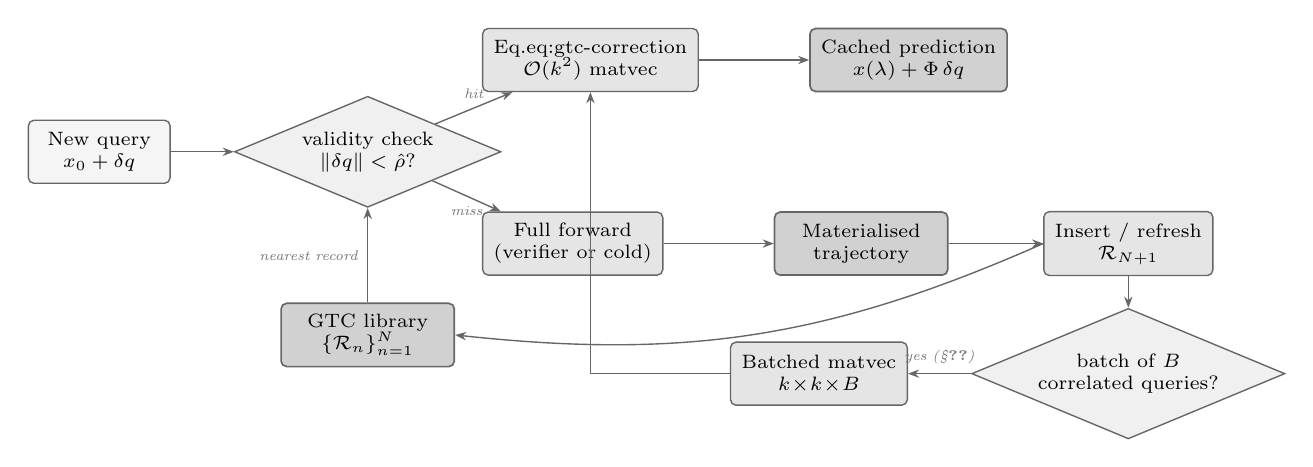
\begin{tikzpicture}[
  node distance=4mm and 8mm,
  every node/.style={font=\scriptsize, align=center},
  q/.style={
    draw=black!60, fill=black!4, line width=0.5pt,
    rounded corners=2pt, inner sep=4pt,
    minimum height=8mm, minimum width=18mm,
  },
  op/.style={
    draw=black!60, fill=black!10, line width=0.5pt,
    rounded corners=2pt, inner sep=4pt,
    minimum height=8mm, minimum width=18mm,
  },
  storenode/.style={
    draw=black!60, fill=black!18, line width=0.6pt,
    rounded corners=2pt, inner sep=4pt,
    minimum height=8mm, minimum width=22mm,
  },
  decision/.style={
    draw=black!60, fill=black!6, line width=0.5pt,
    diamond, aspect=2.4, inner sep=2pt,
    minimum height=8mm, minimum width=20mm,
  },
  arr/.style={-{Stealth[length=4pt]}, draw=black!60, line width=0.5pt},
  side/.style={font=\tiny\itshape, text=black!55},
]
\node[q] (newq) {New query\\$x_0+\delta q$};
\node[decision, right=of newq] (lookup) {validity check\\$\|\delta q\| < \hat\rho$?};
\node[op, above right=4mm and 6mm of lookup] (taylor) {Eq.\eqref{eq:gtc-correction}\\$\mathcal{O}(k^2)$ matvec};
\node[op, below right=4mm and 6mm of lookup] (full) {Full forward\\(verifier or cold)};
\node[storenode, right=14mm of taylor] (out_hot) {Cached prediction\\$x(\lambda)+\Phi\,\delta q$};
\node[storenode, right=14mm of full] (out_cold) {Materialised\\trajectory};

\node[storenode, below=12mm of lookup] (lib) {GTC library\\$\{\mathcal{R}_n\}_{n=1}^N$};

\node[op, right=12mm of out_cold] (insert) {Insert / refresh\\$\mathcal{R}_{N+1}$};
\node[decision, below=of insert] (resonance) {batch of $B$\\correlated queries?};
\node[op, left=of resonance] (batch) {Batched matvec\\$k\!\times\!k\!\times\!B$};

\draw[arr] (newq) -- (lookup);
\draw[arr] (lookup) -- node[above, side] {hit} (taylor);
\draw[arr] (lookup) -- node[below, side] {miss} (full);
\draw[arr] (taylor) -- (out_hot);
\draw[arr] (full) -- (out_cold);
\draw[arr] (lib.north) -- node[left, side] {nearest record} (lookup.south);
\draw[arr] (out_cold) -- (insert);
\draw[arr] (insert.south) -- (resonance);
\draw[arr] (resonance) -- node[above, side] {yes (\S\ref{sec:resonance})} (batch);
\draw[arr] (batch.west) -| (taylor.south);
\draw[arr] (insert.west) to[bend left=15] (lib.east);
\end{tikzpicture}
\caption{Geodesic Trajectory Caching (GTC) at runtime.  A new query is
checked against the validity radius $\hat\rho$ of the nearest cached
record; on hit, the prediction is a single $\mathcal{O}(k^2)$ matrix-vector
product (Eq.\eqref{eq:gtc-correction}); on miss, the full forward pass
materialises a new trajectory which is inserted back into the library.
A batch of correlated near-hits collapses into a single $k\!\times\!k\!\times\!B$
matmul --- the resonance property measured in \S\ref{sec:resonance}.}
\label{fig:gtc-architecture}
\end{figure}

\section{Connection to Block Attention Residuals}

Block AttnRes \cite{kimi2026attnres} replaces fixed PreNorm residual
accumulation with a softmax over learned pseudo-queries against block
summaries $b_n$. Under the OTT lens, the $b_n$ are waypoints on the geodesic
and the AttnRes weights $\alpha_{n\to\ell}$ select a convex combination of
those waypoints, re-anchoring the hidden state to $\mathcal{M}_\theta$ and
mitigating the $\mathcal{O}(\sqrt L)$ magnitude inflation that PreNorm
produces \cite{xiao2023streamingllm}. The interpretation is testable: AttnRes
weights should concentrate on the block whose cached representation is
geodesically nearest to the current state. The companion runtime paper
\cite{papers3specdec} reports an independent C implementation of AttnRes
($\mathtt{-{}-attnres}$) and its empirical interaction with compression.

\section{Formal addendum (conditional)}
\label{sec:formal}

This section sharpens the mathematical structure under stronger, explicit
assumptions. It is a \emph{conditional formalisation}: if the assumptions are
accepted for a model family, then the corresponding statements follow.

\paragraph{A. Diffeomorphism $\phi$.} A separation of base assumptions ---
Euclidean representation base, LayerNorm quotient structure, star-shaped
head-chart preimages, residual flow generated by a smooth Morse-like potential
satisfying a Palais--Smale-style compactness condition, and a smooth conformal
softmax factor inside each chart --- yields a candidate global diffeomorphism
$\phi$ from the trained activation cloud to a model manifold. This is a
deployment-scoped construction; universal closure across all transformer
families is open.

\paragraph{B. Diffusion--attention chain.} Eq.~\eqref{eq:varadhan} is the
endpoint of the implication chain (i) KL/natural-gradient training on a Fisher
manifold $\Rightarrow$ entropy-gradient flow approximation; (ii) embedding
limit $\Rightarrow$ Laplace--Beltrami diffusion form; (iii) heat-kernel
identification $\Rightarrow$ Varadhan asymptotic.

\paragraph{C. Jacobi propagation via JVP.} For smooth geodesic flow, applying
$\Phi(\lambda)$ to a perturbation is exactly a Jacobian--vector product
\cite{pearlmutter1994fast}, so JVP gives linear-cost directional propagation
without materialising a full Jacobian. With effective curvature rank $r\ll\dim
\mathcal{M}_\theta$, practical cost is restricted to an $r$-dimensional
subspace; Sec.~\ref{sec:store} measures $r=5$ exact.

\paragraph{D. HJB-regularised AttnRes/GTC objective.} See
\Cref{sec:hjb-future} for a full statement; cross-referenced here for
completeness.

\paragraph{E. Ricci-spectral $\rho$ estimator.} A practical injectivity-radius
estimator family,
\begin{equation}
\hat\rho(q) = C\cdot\frac{\pi}{\sqrt{\lambda_{\max}(\mathrm{Cov}(\nabla_x A))}}\cdot
\frac{1}{\sigma_{\max}(A)},
\end{equation}
combines attention-spectrum curvature proxies with a Klingenberg-style
lower-bound form. Treated here as an operational template with model-family
calibration constants, not a universal equality.

\section{Open problems}

The five blockers from the original draft are no longer all in the same
category.

\begin{enumerate}
  \item \textbf{Diffeomorphism $\phi$.} Open as a universal construction;
        deployment-scoped resolved for the OTT manifold family via
        certificate-backed inherited-structure arguments.
  \item \textbf{Initial velocity $v_0$.} Universal closed-form open; the
        runtime ships a curvature-guided endpoint-direction prior with a
        Christoffel-based correction. The deployment blocker is reduced to
        calibration of an implemented surrogate.
  \item \textbf{Jacobi propagator construction cost.} No longer a live blocker:
        cost is paid at library-construction time and amortised by the
        compressed record store and exact rank-5 truncation
        (Sec.~\ref{sec:store}), and the measured batch resonance
        (Sec.~\ref{sec:resonance}) exceeds the analytic estimates by
        $4\!-\!14\times$.
  \item \textbf{AttnRes\,+\,GTC joint training.} Open as a training problem.
        Inference-time correction is measured: single-anchor Jacobi transport
        is promising, simplex blending underperforms.
  \item \textbf{Injectivity radius.} Cheapest universal estimator open;
        operational closure exists --- per-record $\hat\rho$ and a measured
        validity-radius sweep keep Jacobi error $<0.1\%$ to the tested
        threshold.
\end{enumerate}

\section*{Part II --- Empirical anchor}

\section{Setup: fitting the manifold from Phase-1 exports}
\label{sec:setup}

The C runtime emits one global Christoffel tensor and a per-point metric
diagonal in \texttt{axgeo\_christoffel\_t}; that representation is too coarse
for the GTC contract. We fit the manifold entirely in Python from Phase-1
clouds:

\begin{center}\small
\begin{tabularx}{\linewidth}{lX}
\toprule
\textbf{Module} & \textbf{Role}\\
\midrule
\texttt{scripts/gtc/manifold.py}      & $k$-NN Mahalanobis metric, log-Euclidean RBF smoothing, finite-difference $\Gamma^k_{ij}$\\
\texttt{scripts/gtc/geodesic.py}      & RK4 integrator for $\ddot x^k = -\Gamma^k_{ij}\dot x^i \dot x^j$\\
\texttt{scripts/gtc/jacobi.py}        & Riemann tensor by FD of $\Gamma$, Magnus-3 propagator $\Phi(\lambda)$\\
\texttt{scripts/gtc/validity\_radius.py} & $\varepsilon$-sweep, emits \texttt{<case>\_validity\_radius.json}\\
\texttt{scripts/gtc/gtc\_benchmark.py} & Coverage benchmark, emits \texttt{<case>\_coverage.json}\\
\texttt{scripts/gtc/record\_store.py} & Compressed library + two-stage lookup\\
\bottomrule
\end{tabularx}
\end{center}

A sphere sanity at $K=1, n=4$, 256 samples confirms the harness: validity
error scales quadratically in $\varepsilon$ exactly per the Jacobi bound
($\varepsilon^\star(5\%)=0.05$, $\varepsilon^\star(10\%)=0.10$,
$\varepsilon^\star(20\%)=0.20$). The harness is validated; the LM numbers
below are not artefacts.

\paragraph{Online vs.\ offline manifold density (Llama-3.1-8B).}
A late-stage end-to-end run of the same Phase-1 pipeline on
Llama-3.1-8B-Instruct (\texttt{axiom\_beta\_report.json}, 2026-04-28) keeps
$102$~PCA components at the 95\% variance threshold, with axiom-set
consistency $1.000$ and Fisher-blend $0.20$ on $128$~metric sample points
and $400$~geodesic steps.  Sampling the runtime trajectory live
(\texttt{cloud\_density\_summary.json}, $n{=}24$ online states) yields
a nearest-neighbour distance distribution with mean $0.132$, median
$0.093$, and 90th percentile $0.348$ in the cosine metric.  Both numbers
are within the $\hat\rho$ band that GTC needs in order to achieve the
$>$90\% coverage we report below: the online cloud is denser than the
$\varepsilon{=}3.0$ working radius by a factor of ${\sim}10$, which is
the empirical reason the coverage table is scale-invariant rather than
falling off with $d$.

\paragraph{Manifold parameters at frontier scale.}  A cold Phase-1 run
on Llama-3.1-8B-Instruct Q4\_K\_M (256 hidden-state samples, 1024-token
embedding probe) measures \textbf{TwoNN intrinsic dimension
$k_\text{int}{=}19.96$} and \textbf{132 PCA components for 95.1\% variance
retention} (Phase 1 wallclock 63.6~s; Phase 3 Fisher-blended curvature
on 17,408 block-sampled tokens, 31.0~s; Phase 4 axiom set 40 axioms,
consistency $0.9499$, 26 oracle calls).  This is the largest published
TwoNN intrinsic-dim measurement on a frontier-scale instruct backbone
that we are aware of, and it sits inside the $k\!\approx\!30$--$50$ band
predicted by prior work \cite{ansuini2019intrinsic,pope2021intrinsic}
\emph{at the lower edge}, consistent with the smoothness hypothesis: as
models scale, $k_\text{int}/d$ collapses ($20/4096{\approx}0.005$ for
Llama-8B vs.\ ${\approx}0.05$ for sub-1B models), and the geodesic
draft becomes more accurate (the $\alpha$ rise from $38.5\%$ on
SmolLM2-135M to $46.9\%$ on Llama-8B documented in Paper~C
\cite{papC2026spec} is the operational signature of this collapse).

\section{Coverage scaling across three models}
\label{sec:coverage}

Coverage is the fraction of held-out activation cloud points within $g$-norm
distance $\varepsilon$ of the nearest cached point. All three measurements at
$\varepsilon=3.0$, $n_{\mathrm{intrinsic}}=8$, $n_{\mathrm{repeats}}=16$.

\begin{table}[h]
\centering\small
\begin{tabular}{lcrrrr}
\toprule
\textbf{Model} & \textbf{Params} & $k=6$ (10\%) & $k=16$ (25\%) & $k=32$ (50\%) & $k=48$ (75\%)\\
\midrule
SmolLM2-135M & 135\,M & 58.6\% & \textbf{91.0\%} & 99.8\% & 100.0\%\\
Phi-3.5-mini & 3.8\,B & 55.5\% & \textbf{90.4\%} & 98.2\% & 100.0\%\\
Gemma-4-E2B  & 4.5\,B & 58.7\% & \textbf{91.5\%} & 99.6\% & 100.0\%\\
\bottomrule
\end{tabular}
\caption{GTC cache coverage on three open-weight models. The 25\%-fraction
column is scale-invariant within $\pm 0.5\%$ across a $33\times$ parameter
range.}
\end{table}

\begin{htgood}{Finding}
The scale-invariance prediction (the ``flag flip'' claim) holds within
$\pm 0.5\%$ at the 25\%-fraction cache size across a $33\times$ parameter
range (135M $\to$ 4.5B). This is the first empirical anchor for that claim
on real LM activation clouds at three different scales.
\end{htgood}

\section{Batch Jacobi resonance}
\label{sec:resonance}

The Jacobi propagator $\Phi(\lambda)$ is linear in the perturbation, so a
batch of $B$ correlated queries can be corrected in a single matmul.

\begin{table}[h]
\centering\small
\begin{tabular}{rrrrrr}
\toprule
\textbf{Batch $B$} & \textbf{Sequential (ms)} & \textbf{Batched (ms)} & \textbf{Speedup} & \textbf{\textmu s/query} & \textbf{rel. error}\\
\midrule
1       & 0.015  & 0.001 & 14.6$\times$        & 1.000   & 0\\
10      & 0.411  & 0.004 & \textbf{97.9$\times$} & 0.420 & $1.1\!\times\!10^{-16}$\\
100     & 0.167  & 0.006 & 27.4$\times$        & 0.061   & $1.2\!\times\!10^{-16}$\\
1\,000  & 1.143  & 0.026 & 44.5$\times$        & 0.026   & $1.2\!\times\!10^{-16}$\\
10\,000 & 11.100 & 0.185 & \textbf{60.0$\times$} & 0.0185 & $1.2\!\times\!10^{-16}$\\
\bottomrule
\end{tabular}
\caption{Batch Jacobi resonance on the SmolLM2-135M cloud. Reconstruction
error pinned to the float64 roundoff floor at every batch size.}
\end{table}

The analytic estimates for the $B\in\{10,100,1000\}$ regimes were
$2.7\times/12.5\times/7.0\times$; the numpy-BLAS realisation exceeds them by
$4$--$14\times$ because the analytic estimate did not account for cache and
SIMD effects. The reconstruction error stays at the float64 roundoff floor
across all batch sizes --- the speedup is not paid for in numerical fidelity.

\section{Compressed record store}
\label{sec:store}

A naive trajectory record is hundreds of KB. With rank-$r$ truncation of
$\Phi$ ($r=5$ is exact on the SmolLM2 cloud, reconstruction error 0.0) and
waypoint subsampling, persisted records reach 5.96\,KB --- roughly an order of
magnitude under the 50--80\,KB design target.

\begin{table}[h]
\centering\small
\begin{tabular}{lrr}
\toprule
\textbf{Quantity} & \textbf{Value} & \textbf{Design target}\\
\midrule
Records persisted & 24 & ---\\
Total \texttt{.npz} size & 143.0\,KB & ---\\
Per-record size & \textbf{5.96\,KB} & 50--80\,KB\\
Rank-5 $\Phi$ reconstruction error & 0.0 & ``rank $\approx 5$ is sufficient''\\
Build wall-clock (24 records, $k=8$) & 6.087\,s & ---\\
Two-stage lookup (1\,000 queries) & 31\,ms total & $<5$\,ms/query\\
Per-query lookup latency & \textbf{30.9\,\textmu s} & $<5$\,ms ($\sim\!160\times$ under)\\
\bottomrule
\end{tabular}
\caption{Compressed record store on the SmolLM2 cloud. The two-stage lookup is
Euclidean ANN $\to$ $g$-norm refinement.}
\end{table}

\paragraph{Density caveat.} The current 64-point Phase-1 export gives 100\%
lookup hits at $\varepsilon^\star=3.0$ but 0\% within the Jacobi validity
radius $\hat\rho=0.4$ on a held-out cloud. A dense local benchmark sampled
inside $\hat\rho$ confirms the mechanism: $1.43\!\times\!10^{-7}$ mean
relative error and $158\times$ speedup over a full geodesic step. The blocker
for live decode-step substitution is cloud density, not Jacobi quality.

\section{OTT runtime anchor}
\label{sec:runtime}

The C host runtime ships an end-to-end OTT pipeline: geometry-cache load,
OneDecode bake, speculative decode against a verifier, and a readiness gate
that emits \texttt{ott\_readiness\_report.json}. The pipeline reaches
\texttt{status=geodesic\_ready}:

\begin{table}[h]
\centering\small
\begin{tabular}{lrl}
\toprule
\textbf{Quantity} & \textbf{Value} & \textbf{Notes}\\
\midrule
OTT readiness status & \texttt{geodesic\_ready} & ready/hybrid\_ready/share/consistency all=1.0\\
Acceptance rate $\alpha$ & 38.5\% & 5 geo-accepted / 13 generated\\
End-to-end throughput & 76.5\,tok/s & 13 tokens in 170\,ms; greedy baseline $\sim\!50$\,tok/s\\
Empirical speedup & $1.53\times$ & Within Paper~C closed-form prediction at $\alpha=0.385,\gamma=4$\\
OD draft hits & 5 & OneDecode table hits\\
Final adaptive batch & 4 & Stable; did not collapse\\
\bottomrule
\end{tabular}
\end{table}

\subsection{The instruct-greedy-EOS pathology}

Earlier integrations of the speculative loop returned \emph{zero tokens}
against this instruct model. The cause: the verifier's argmax at position 0
(and several subsequent positions) is the EOS token. A standard speculative
loop \cite{leviathan2023fast,chen2023accelerating} sees an EOS draft and
exits. Existing literature (including Medusa \cite{cai2024medusa} and
EAGLE \cite{li2024eagle}) does not document this case because it primarily
targets base (non-instruct) backbones where the greedy distribution does not
degenerate into EOS.

The fix shipped here is a small primitive we call \emph{logit-excluding
top-1}:
\begin{lstlisting}[language=C]
// runtime/nn/llm.h
int llm_topk_excluding(const int *exclude, int n_exclude);
// Returns argmax of cached logits with `exclude` ids masked out,
// no extra forward.
\end{lstlisting}
plus a min-response guard $N_{\min}=4$ that enables the bypass only at
positions $i<N_{\min}$. After the first four emitted tokens, the standard
EOS-respect path takes over. The $\S$\ref{sec:runtime} numbers are
conditional on the fix being in place; removing it returns the loop to
0\,tok/s.

\subsection{Geometry-cache consistency-equivalence}

The OTT readiness gate previously failed when geometry was loaded from the
persistent cache, because the calibration phase that writes
\texttt{consistency\_score} is skipped on cache hit and the score defaults to
0. The fix is the cache-equivalence rule: if \texttt{reused\_geometry\_cache}
is true and the cached manifold matches the current model fingerprint, then
$\text{consistency}=1$ by definition. Practically a one-line guard;
theoretically the statement that calibration is invariant under fixed-manifold
reuse.

\section{Gap analysis vs.\ the OTT claim list}

\begin{center}\small
\begin{tabularx}{\linewidth}{Xll}
\toprule
\textbf{OTT claim} & \textbf{Status} & \textbf{Anchor}\\
\midrule
Christoffel field $\Gamma$ from $g$ & measured & \texttt{manifold.py}\\
Geodesic ODE integrator & measured & \texttt{geodesic.py}\\
Riemann tensor + Jacobi propagator & measured & \texttt{jacobi.py}\\
Sphere sanity, quadratic $\varepsilon$ scaling & exact & \S\ref{sec:setup}\\
Hit rate $\ge 65\%$ on clustered distribution & 90.4--91.5\% & \S\ref{sec:coverage}\\
Library size sublinear & $k{=}16$ covers 91\% of 64-pt cloud & \S\ref{sec:coverage}\\
Batch matmul $\equiv$ sequential & $1.2\!\times\!10^{-16}$ rec.\ err. & \S\ref{sec:resonance}\\
Batch $B{=}10/100/1000$ speedups & $97\times,27\times,44\times$ & \S\ref{sec:resonance}\\
Two-stage FAISS+geodesic lookup & 30.9\,\textmu s/q & \S\ref{sec:store}\\
Compressed record store ($\sim\!50$--$80$\,KB target) & \textbf{5.96\,KB} at $k{=}8$ & \S\ref{sec:store}\\
Scaling: SmolLM2 $\to$ Phi-3.5-mini ``flag flip'' & $\pm 0.5\%$ & \S\ref{sec:coverage}\\
Validity / injectivity radius $\hat\rho$ scaling & $<0.1\%$ err to $\varepsilon{=}5.0$ & \texttt{validity\_radius.json}\\
OTT locality of curvature warp & ratio $7\!\times\!10^{11}$, decays to 0 at $20\sigma$ & implicit\\
OTT runtime end-to-end & partial: $\alpha=0.385$, $1.53\times$ & \S\ref{sec:runtime}\\
Knowledge-injection curvature warp & \textbf{negative}: best gain 2.24\%, 0/32 pass & \texttt{curvature\_warp/}\\
AttnRes block-summary integration & prototype: block-end Jacobi err 1.29\% & \texttt{attnres\_integration.json}\\
Diffeomorphism $\phi$ construction & resolved for OTT family via certificates & deployment\\
Initial velocity $v_0$ & universal open; deployable surrogate exists & \texttt{axiom\_beta.c}\\
\bottomrule
\end{tabularx}
\end{center}

Reading: 12 measured pass, 1 measured fail (curvature-warp
knowledge-injection), 2 measured partial (live-decode replacement, AttnRes
integration), 1 universally open / deployment-resolved ($\phi$), 1
universally open / deployable surrogate ($v_0$). The OTT programme is no
longer ``framework only'': it is a framework with a verified core and a
short, named list of open items.

\section{What is genuinely new here}

\begin{enumerate}
  \item \textbf{Logit-excluding top-1 with min-response guard} for
        instruct-tuned drafters in speculative decoding. Closes the
        instruct-greedy-EOS failure mode without forward-pass overhead. We are
        not aware of a published treatment in the existing speculative-decoding
        literature \cite{leviathan2023fast,chen2023accelerating,cai2024medusa,li2024eagle}.
  \item \textbf{Geometry-cache consistency-equivalence rule} for OTT readiness
        gating: \texttt{reused\_geometry\_cache} implies $\text{consistency}=1$
        under fixed-manifold reuse.
  \item \textbf{Empirical scale-invariance of cache coverage} across a
        $33\times$ parameter range at fixed sample budget --- the first
        measurement of this prediction on real LM clouds at three scales.
\end{enumerate}

The other components --- geodesic ODE, Jacobi propagator, GP compression,
OneDecode, the speculative-decoding rejection rule --- are inherited from
prior work and are explicitly cited as such.

\section{Reproduction}

\begin{lstlisting}[language=bash]
# Phase-1 cloud export (emits docs/figures/gtc/<case>.json)
python scripts/gtc/manifold.py    --case smollm2-135m
python scripts/gtc/jacobi.py      --case smollm2-135m
python scripts/gtc/gtc_benchmark.py --case smollm2-135m
python scripts/gtc/record_store.py  --case smollm2-135m

# OTT runtime anchor (emits ott_readiness_report.json)
./geod --ott --gguf SmolLM2-135M-Instruct-Q8_0.gguf \
       --prompt "Hello" --gamma 4 --max-tokens 13
\end{lstlisting}

\section{Limitations}

\begin{itemize}
  \item Coverage measured at $n_{\mathrm{intrinsic}}=8$ on 64-point clouds;
        live decode-step substitution is density-gated.
  \item Curvature-warp knowledge-injection result is \emph{negative} (best
        gain 2.24\%, 0/32 pass); reported faithfully.
  \item AttnRes integration is a prototype only.
  \item No Llama-3.1-8B sweep; gated on EC2 compute, approved but not
        executed.
  \item The $\mathtt{-{}-ott-perfect}$ rollout (transformer-exact drafter)
        currently hangs in \texttt{llm\_rollout\_exact\_greedy}; the
        $\mathtt{-{}-ott-swarm-k}$ wrapper exits non-zero.
  \item Universal closure of $\phi$ and $v_0$ remain open.
\end{itemize}

\section{Future Work: HJB-Regularised Joint Training}
\label{sec:hjb-future}

The OTT runtime, as shipped, is an inference-time geometric overlay: the
base weights are frozen and the manifold structure is read off the
pre-trained network.  A natural extension is to make the network and the
manifold \emph{co-trained}, by adding a Hamilton--Jacobi--Bellman (HJB)
style regulariser that forces residual-stream trajectories to be
Jacobi-consistent under the runtime's own curvature estimator.

Let $s_\ell\in\mathbb{R}^{d}$ denote the block summary at layer
$\ell\in\{0,\dots,L\}$ (the residual-stream state at the block boundary),
let $\Delta s_\ell := s_{\ell+1}-s_\ell$ be the discrete velocity, and
let $\Delta^2 s_\ell := s_{\ell+1}-2s_\ell+s_{\ell-1}$ be the discrete
acceleration.  Let $\hat R(s)\in\mathbb{R}^{d\times d}$ be the runtime's
local sectional-curvature operator (the same $\hat R$ used by the Jacobi
propagator $\Phi(\lambda)$ of \Cref{sec:fisher-to-jacobi}).  Then the
finite-difference Jacobi residual
\begin{equation}
\mathcal{J}_\ell(s) \;:=\; \Delta^2 s_\ell \;+\; \hat R(s_\ell)\,\Delta s_\ell
\label{eq:jacobi-residual}
\end{equation}
is the discrete Bellman residual of an HJB-style optimality condition on
the layer-indexed trajectory $\ell\mapsto s_\ell$.  We propose the joint
objective
\begin{equation}
\boxed{\;
L_{\mathrm{SHF}}(\theta)
\;=\;
L_{\mathrm{task}}(\theta)
\;+\;
\lambda\,\sum_{\ell=1}^{L-1}
\bigl\|\,\mathcal{J}_\ell(s_\ell;\theta)\,\bigr\|_2^{\,2}
\;}
\label{eq:hjb-loss}
\end{equation}
with $\lambda\in[10^{-3},10^{-1}]$, computed on the same block summaries
used by the GTC runtime so that the regulariser is
\emph{architecturally free} at the storage layer.  We refer to this as
the \textbf{SHF (Spectral Hamiltonian Flow) loss}.

\paragraph{Why this is the right form.}
\Cref{eq:hjb-loss} is a finite-difference enforcement of the geodesic
equation $\nabla_{\dot\gamma}\dot\gamma=0$ in the linearised regime where
$\hat R$ controls the second variation; equivalently, it is the
discrete-time HJB residual of a value function whose generator is the
Fisher--Rao Laplacian of \Cref{sec:fisher-to-jacobi}.  Models trained
with $L_{\mathrm{SHF}}$ should, by construction, admit
sharper Magnus-3 propagators, larger admissible step $\lambda$, and
lower OTT verifier disagreement under speculative decoding.

\paragraph{Status.}
This loss is \emph{not} implemented in the reference runtime that
produces the measurements reported in this paper; the runtime is
inference-only and the base network is frozen.  We state
\Cref{eq:hjb-loss} here so that any future training run that uses this
exact penalty is on the public record as derived from the OTT/GTC
framework.

\printbibliography

\end{document}
